% !TeX program = pdflatex
% The Clock That Never Ticks — a machine-checked path from the dilogarithm to
% quantum speed limits in Lean 4.  Story-driven structure: each section is the
% question that produced it; the narrative advances by turns to the ending.
% Build: pdflatex clock-never-ticks.tex  (twice, for refs)
% Verified against the Lean source 2026-06-13 (lake build Dilog QSL, 8426 jobs, exit 0;
% #print axioms on every named theorem -> propext, Classical.choice, Quot.sound only).
% Toolchain v4.30.0-rc2, Mathlib pin 701fb6e9.

\documentclass[11pt]{article}
\usepackage[T1]{fontenc}
\usepackage{lmodern}
\DeclareUnicodeCharacter{2082}{\ensuremath{_2}}
\DeclareUnicodeCharacter{208A}{\ensuremath{_+}}
\usepackage{amsmath,amssymb,amsthm,booktabs,graphicx,hyperref}
\usepackage{xurl}
\usepackage[table]{xcolor}
\definecolor{ggteal}{HTML}{1B6F8C}
\definecolor{ggband}{HTML}{DCE7EB}
\definecolor{ggamber}{HTML}{E08A1E}
\usepackage[margin=1in]{geometry}
\usepackage{microtype}
\usepackage{float}
\usepackage[section]{placeins}
\usepackage[most]{tcolorbox}
\usepackage{tikz}
\usetikzlibrary{arrows.meta,positioning}
\setlength{\emergencystretch}{2em}
\graphicspath{{figures/}}
\newtheorem{theorem}{Theorem}
\newtheorem{proposition}{Proposition}
\newtheorem{lemma}{Lemma}
\newtheorem{definition}{Definition}
\newtheorem{remark}{Remark}
\newcommand{\lean}[1]{\texttt{#1}}
\newcommand{\R}{\mathbb{R}}
\newcommand{\N}{\mathbb{N}}
\newcommand{\C}{\mathbb{C}}
\newcommand{\Li}{\mathrm{Li}_2}
\newcommand{\Cl}{\mathrm{Cl}_2}
\DeclareMathOperator{\Lrog}{L}
\hypersetup{colorlinks=true,linkcolor=ggteal,citecolor=ggteal,urlcolor=ggteal}
\newtcbox{\keybox}{on line,boxrule=0.9pt,colframe=ggteal,colback=ggband!40,
  arc=3pt,left=8pt,right=8pt,top=5pt,bottom=5pt}
\newcommand{\keyeq}[1]{\begin{center}\keybox{$\displaystyle #1$}\end{center}}
\newtcolorbox{recipebox}[1]{boxrule=0.9pt,colframe=ggamber,colback=ggband!25,
  arc=3pt,title={\textbf{#1}},fonttitle=\small,fontupper=\small}

\title{\bf The Clock That Never Ticks\\[4pt]
  \large\normalfont A machine-checked path from the dilogarithm\\
  to quantum speed limits in Lean~4}
\author{Carles Mar\'in\thanks{Formalized with AI assistance (Claude, Anthropic); the
mathematics and all claims are the author's responsibility. The methodology and the
exact boundary of the contribution are discussed in Section~\ref{sec:boundary}.}\\[3pt]
  \normalsize Independent researcher\\
  \normalsize \texttt{karlesmarin@gmail.com}}
\date{June 2026}

\begin{document}
\maketitle

\begin{abstract}
Mathlib's source contains a comment referring to the dilogarithm $\Li$ --- a function the
library does not have. We fill that hole and follow the questions where they lead. The
result is a \lean{sorry}-free Lean~4 development ($\sim$1\,500 lines over Mathlib)
containing, to the best of our knowledge, several firsts in any proof assistant: the
real dilogarithm with Euler's reflection identity, Landen's transformation, the
duplication formula, and the golden-ratio ladder
$\Li(1/\varphi^2)=\pi^2/15-\ln^2\varphi$, $\Li(1/\varphi)=\pi^2/10-\ln^2\varphi$
(derived from a $3\times 3$ linear system --- no five-term relation needed); the Rogers
value $\Lrog(1/\varphi^2)=\pi^2/15$, equivalently the Lee--Yang effective central charge
$c_{\mathrm{eff}}=2/5$, the simplest thermodynamic-Bethe-ansatz dilogarithm identity;
the Clausen function $\Cl$ and \emph{Catalan's constant} $G=\Cl(\pi/2)$; the
\emph{Fej\'er--Jackson inequality} $\sum_{k=1}^{M}\sin(k\theta)/k>0$ on $(0,\pi)$; the
positivity $\Cl(\theta)\ge\sin(\theta)/2$ by an asymptotics-free Abel summation; and the
\emph{Margolus--Levitin} and (an $L^1$ form of the) \emph{Mandelstam--Tamm} quantum
speed limits. The pieces assemble into the ending the title promises: the quantum state
with populations $\propto 1/n^2$ on equally spaced energy levels has \emph{infinite}
mean energy and \emph{infinite} energy variance --- both textbook speed limits say
nothing --- and yet \emph{never} reaches a state orthogonal to itself, because its
autocorrelation is $\tfrac{6}{\pi^2}\Li(e^{-i\theta})$ and the dilogarithm has no zero
on the unit circle. A clock with an unbounded energy budget that never ticks. We are
exact about the boundary: every identity here is classical (Euler, Landen, Clausen,
Fej\'er, Jackson, Mandelstam--Tamm, Margolus--Levitin); the contribution is the
machine-checked development and its assembly. Every named theorem depends only on the
three standard axioms.
\end{abstract}

\medskip
\noindent\emph{How to read this paper.} It is written as the story of six questions.
Five of them form a chain --- each section opens with its question and closes by handing
the reader the next. The sixth (\emph{how fast can a quantum state evolve?}) did
\emph{not} grow out of the chain: it was born independently, from asking which part of
the ``universe as a computer'' metaphor is an actual theorem, and it \emph{crossed} the
chain at its end. Figure~\ref{fig:map} is the honest map, crossing included. If you read
only one thing, read Theorem~\ref{thm:clock} and Figure~\ref{fig:clock}; the Lean
inventory is Table~\ref{tab:inventory}, and reproduction takes three commands
(Appendix~\ref{app:repro}).

\begin{figure}[h]
\centering
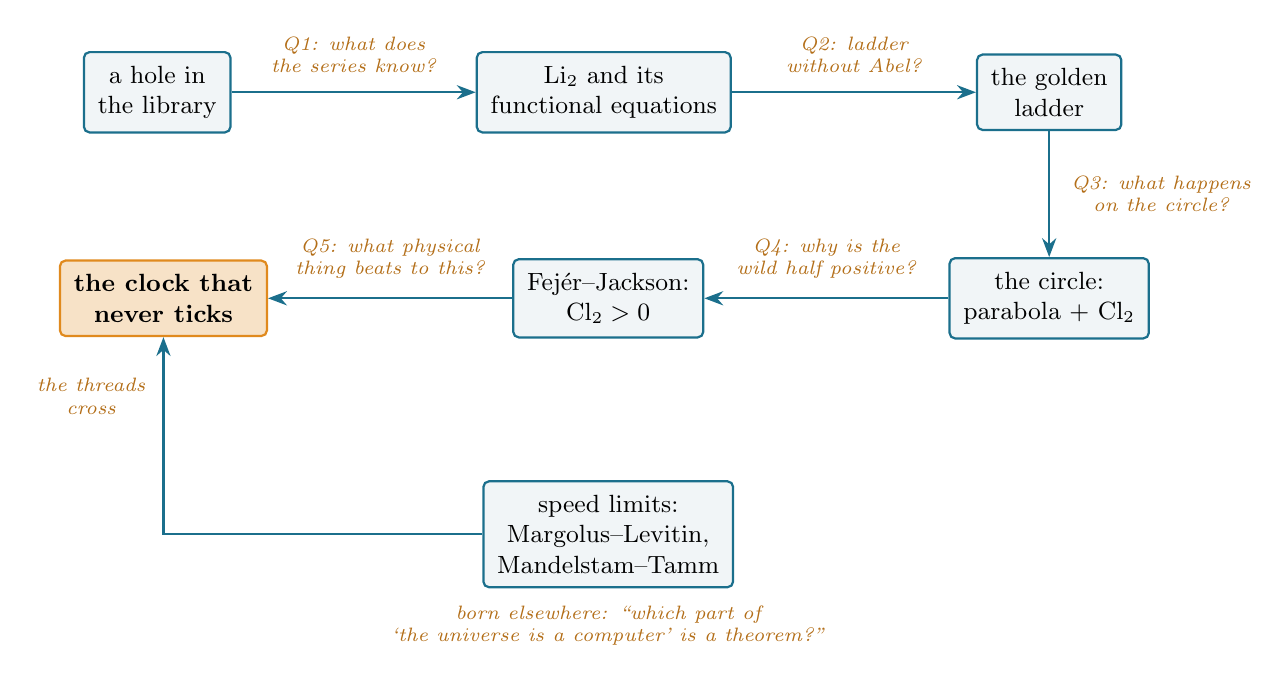
\begin{tikzpicture}[
  obj/.style={draw=ggteal, thick, rounded corners=2pt, fill=ggband!40,
    align=center, font=\small, inner sep=5pt},
  q/.style={font=\scriptsize\itshape, text=ggamber!80!black, align=center},
  arr/.style={-{Stealth[length=2.4mm]}, thick, ggteal}]
\node[obj] (hole) {a hole in\\the library};
\node[obj, right=31mm of hole] (li2) {$\Li$ and its\\functional equations};
\node[obj, right=31mm of li2] (gold) {the golden\\ladder};
\node[obj, below=16mm of gold] (circle) {the circle:\\parabola $+$ $\Cl$};
\node[obj, left=31mm of circle] (pos) {Fej\'er--Jackson:\\$\Cl>0$};
\node[obj, left=31mm of pos, fill=ggamber!25, draw=ggamber] (clock)
  {\textbf{the clock that}\\\textbf{never ticks}};
\node[obj, below=18mm of pos] (qsl) {speed limits:\\Margolus--Levitin,\\Mandelstam--Tamm};
\node[q, below=1mm of qsl] {born elsewhere: ``which part of\\`the universe is a
  computer' is a theorem?''};
\draw[arr] (hole) -- node[q, above=1.2mm] {Q1: what does\\the series know?} (li2);
\draw[arr] (li2) -- node[q, above=1.2mm] {Q2: ladder\\without Abel?} (gold);
\draw[arr] (gold) -- node[q, right=1.5mm] {Q3: what happens\\on the circle?} (circle);
\draw[arr] (circle) -- node[q, above=1.2mm] {Q4: why is the\\wild half positive?} (pos);
\draw[arr] (pos) -- node[q, above=1.2mm] {Q5: what physical\\thing beats to this?} (clock);
\draw[arr] (qsl) -| node[q, left=1mm, pos=0.85] {the threads\\cross} (clock);
\end{tikzpicture}
\caption{The honest map. The dilogarithm thread runs along the top and back; the
quantum thread (bottom) was born independently and \emph{crossed} it at the end ---
the crossing, not the chain, is where the title theorem lives. Every node is a block of
\lean{sorry}-free Lean.}
\label{fig:map}
\end{figure}

\section{The question that starts it: why does the library cite a function it does not
have?}\label{sec:intro}

Few functions have been discovered as many times as the dilogarithm. Euler wrote down
its series in the 1760s; within a century it had been met again by Spence, by Abel in
the study of its functional equations, by Lobachevsky in the measurement of hyperbolic
space, and by Kummer --- each giving it a different name and a different reason to care.
Two centuries later it reappeared, unbidden, in the finite parts of Feynman integrals
and in the thermodynamics of integrable systems. It is the rare non-elementary function
that now and then consents to a closed form, and the catalogue of those closed forms
reads like a tour of mathematics. So there is something almost comic in the fact that,
in 2026 --- after a decade of one of the most ambitious formalization efforts ever
attempted --- the dilogarithm was not in the library at all. The machines we now use to
certify theorems had never been told what $\Li$ is. They had, however, been told to
mention it.

The file \lean{Mathlib/Analysis/SpecialFunctions/Integrals/LogTrigonometric.lean} of
Mathlib --- the mathematical library of the Lean~4 proof assistant, on which a
substantial part of contemporary formalized mathematics is built --- describes one of
its integrals by referring to the dilogarithm
\[
\Li(x) \;=\; \sum_{n\ge 1}\frac{x^n}{n^2}.
\]
The function itself is absent. Not just from Mathlib: as far as we could determine,
the dilogarithm, the Clausen function, Catalan's constant, the Fej\'er--Jackson
inequality, and every quantum speed limit are absent from \emph{every} proof assistant
(Lean, Rocq/Coq, Isabelle); the existing quantum libraries (CoqQ, SQIR, Isabelle Marries
Dirac) formalize circuits, not dynamical bounds.\footnote{Library and literature checks
performed June 2026: Loogle and \lean{grep} over Mathlib (zero \lean{quantum}
declarations; no \lean{dilog}/\lean{polylog}/\lean{Clausen}, and Catalan
\emph{numbers} only); web searches over the Archive of Formal Proofs and the Rocq/Coq
ecosystems. Absence of evidence, with that caveat.}

How does a function this central stay unformalized for a decade of Mathlib? Because it
sits in an odd blind spot: too special to be infrastructure, too analytic to be
algebra, and guarded --- as we will see --- by exactly one genuinely delicate limit. The
genesis of this project was an audit: a fifty-digit numerical verification of the
dilogarithm identities in a recent preprint of Alha~\cite{alha}. Auditing someone
else's dilogarithms sent us to the library for a reference implementation; the library
sent us back empty-handed. We decided to fill the hole, and to keep asking the next
question until the questions stopped. They stopped five sections later, inside a
quantum mechanics problem. This paper is the travelogue.

\section{Q1: what does the series know about its own derivative?}\label{sec:dilog}

\emph{History bead.} The function is Euler's (1768); the reflection identity below is
his. Landen's transformation is from 1780. Everything in this section is classical
(Lewin~\cite{lewin}, Zagier~\cite{zagier}); the Lean is \lean{Dilog/Basic.lean}.

A power series differentiates termwise, and the dilogarithm's derivative collapses to
elementary functions:
\[
\Li'(x) \;=\; \sum_{n\ge1}\frac{x^{n-1}}{n} \;=\; -\frac{\ln(1-x)}{x}
\qquad(\lvert x\rvert<1,\ x\ne 0).
\]
In Lean this single line is the analytic core of the whole development ---
term-by-term differentiation under a geometric majorant
(\lean{hasDerivAt\_tsum\_of\_isPreconnected}), then the Mercator series to identify the
sum. Once the derivative is known, functional equations become mechanical:

\begin{recipebox}{Recipe: a functional equation in three moves}
To prove a combination $F$ of dilogarithms and logarithms is constant on an interval:
(1)~differentiate termwise and check $F'=0$ by chain/product rules plus
\lean{field\_simp; ring}; (2)~conclude $F$ is constant by mean-value machinery
(\lean{constant\_of\_has\_deriv\_right\_zero} on subintervals); (3)~evaluate the
constant as a \emph{boundary limit}. Step (3) is where the one delicate limit of the
subject lives: $\ln x\cdot\ln(1-x)\to 0$ at the endpoint, tamed as
$\big(\ln(1-x)/x\big)\cdot\big(x\ln x\big)\to(-1)\cdot 0$ via the slope
characterization of the derivative and \lean{tendsto\_log\_mul\_rpow\_nhdsGT\_zero}.
Continuity of $\Li$ up to the boundary is the Weierstrass $M$-test
(\lean{continuousOn\_tsum}).
\end{recipebox}

\begin{theorem}[{\lean{Li₂\_add\_Li₂\_one\_sub}, \lean{Li₂\_landen},
\lean{Li₂\_sq}, \lean{Li₂\_one\_half}}]\label{thm:funceq}
On the stated domains,
\begin{align*}
\Li(x)+\Li(1-x) &= \tfrac{\pi^2}{6}-\ln x\,\ln(1-x) && x\in(0,1)\\
\Li(x)+\Li\!\Big(\tfrac{x}{x-1}\Big) &= -\tfrac{1}{2}\ln^2(1-x) && x\in(0,\tfrac12)\\
\Li(x^2) &= 2\big(\Li(x)+\Li(-x)\big) && \lvert x\rvert\le 1\\
\Li(\tfrac12) &= \tfrac{\pi^2}{12}-\tfrac{\ln^2 2}{2}.
\end{align*}
\end{theorem}

Two honesty notes, both visible in the Lean statements. The Landen domain stops at
$x=\frac12$: past it, the argument $x/(x-1)$ leaves the disc of convergence, and a
power-series definition does not analytically continue --- we do not pretend it does.
And the duplication formula needs no calculus at all: it is a pure rearrangement of the
series by even and odd indices (\lean{tsum\_even\_add\_odd}), the formal mirror of how
Euler would have proved it.

\emph{From theory to practice.} The dilogarithm is the standard weight-2 function of
one-loop Feynman integrals and of hyperbolic and $K$-theoretic invariants; textbooks
reach for it constantly. The practical value of formalizing it is modest and specific:
a verified \lean{Li2} with its functional equations --- including the one delicate
boundary limit --- that downstream Lean developments can import rather than re-derive.

\emph{The turn.} Three functional equations in hand, the classical showpieces of the
subject are the golden-ratio evaluations --- and every textbook reaches them through
Abel's five-term relation, a two-variable identity we have \emph{not} formalized.
Are we stuck?

\section{Q2: can the golden ladder be climbed without Abel's relation?}
\label{sec:golden}

\emph{History bead.} The values are Landen's (1780); the two-term sum is from Rogers'
1907 memoir~\cite{rogers}. Their role as a central charge belongs to the thermodynamic
Bethe ansatz of the 1990s~\cite{zamolodchikov,nahm,kirillov}.

The answer is yes, and the key is two arithmetic accidents of the golden ratio
$\varphi=(1+\sqrt5)/2$, both one-liners from $\varphi^2=\varphi+1$:
\[
\frac{1}{\varphi}+\frac{1}{\varphi^2}=1
\qquad\text{and}\qquad
\frac{1/\varphi^2}{1/\varphi^2-1}=-\frac{1}{\varphi}.
\]
The first says $1/\varphi$ and $1/\varphi^2$ are a \emph{reflection pair}; the second
says \emph{Landen maps $1/\varphi^2$ to $-1/\varphi$} --- and note
$1/\varphi^2\approx0.382<\tfrac12$, inside our proven Landen domain. Reflection at
$1/\varphi^2$, Landen at $1/\varphi^2$, duplication at $1/\varphi$: three linear
equations, three unknowns, and \lean{linarith} closes the system.
\keyeq{
\Li\!\Big(\tfrac{1}{\varphi^2}\Big)=\tfrac{\pi^2}{15}-\ln^2\varphi,
\qquad
\Li\!\Big(\tfrac{1}{\varphi}\Big)=\tfrac{\pi^2}{10}-\ln^2\varphi,
\qquad
\Li\!\Big(-\tfrac{1}{\varphi}\Big)=\tfrac{\ln^2\varphi}{2}-\tfrac{\pi^2}{15}.
}
No five-term relation --- a small but pleasant discovery of the formalization process.
In the Rogers normalization $\Lrog(x)=\Li(x)+\tfrac12\ln x\ln(1-x)$ the $\ln^2$ defects
cancel (\lean{rogersL\_inv\_goldenRatio\_sq}, \lean{rogersL\_gold\_sum}):
\[
\Lrog\!\Big(\tfrac{1}{\varphi^2}\Big)=\frac{\pi^2}{15},\qquad
\Lrog\!\Big(\tfrac{1}{\varphi}\Big)+\Lrog\!\Big(\tfrac{1}{\varphi^2}\Big)
=\frac{\pi^2}{6}=\Lrog(1),
\]
and the first, normalized, is the effective central charge of the Lee--Yang
thermodynamic Bethe ansatz, $c_{\mathrm{eff}}=\Lrog(1/\varphi^2)/\Lrog(1)=2/5$ --- to
our knowledge the first TBA dilogarithm identity verified in a proof assistant.

\emph{From theory to practice.} The value $c_{\mathrm{eff}}=2/5$ is the effective central
charge of the Lee--Yang model, a non-unitary minimal CFT whose Yang--Lee zeros have been
observed experimentally in spin systems. The identity formalized here is the simplest
entry of the thermodynamic-Bethe-ansatz dilogarithm table; having one machine-checked
anchors any later formalization of integrable-model thermodynamics.

\emph{The turn.} The ladder spends the function's life \emph{inside} the interval of
convergence. The natural next territory is the boundary itself. What does the series do
on the unit circle?

\section{Q3: what happens on the circle?}\label{sec:circle}

\emph{History bead.} Clausen introduced his function in 1832~\cite{clausen}; Catalan's
constant is from his 1865 memoir, and its irrationality is, famously, still open. The
cosine series below is the Fourier expansion of the Bernoulli polynomial $B_2$, which
Mathlib already owns (\lean{hasSum\_one\_div\_nat\_pow\_mul\_cos}); the Lean of this
section is \lean{Dilog/Clausen.lean}.

On the circle the dilogarithm splits into a tame half and a wild half:
\[
\Li(e^{i\theta}) \;=\;
\underbrace{\sum_{n\ge1}\frac{\cos n\theta}{n^2}}_{\textstyle
  =\;\frac{\pi^2}{6}-\frac{\pi\theta}{2}+\frac{\theta^2}{4}}
\;+\; i\,\underbrace{\sum_{n\ge1}\frac{\sin n\theta}{n^2}}_{\textstyle =\;\Cl(\theta)}
\qquad(\theta\in[0,2\pi]).
\]
The real part is an \emph{elementary parabola}
(\lean{hasSum\_cos\_div\_sq}, from Mathlib's Bernoulli--Fourier machinery at $k=1$).
The imaginary part is not elementary at all: it is the \textbf{Clausen function}, a
genuinely new special function --- the reason this section exists. At the quarter circle
it produces a celebrity:
\[
G \;=\; \Cl\!\Big(\frac{\pi}{2}\Big) \;=\; \sum_{k\ge0}\frac{(-1)^k}{(2k+1)^2}
\;=\;0.9159\ldots,
\]
\textbf{Catalan's constant}, absent --- as far as we could determine --- from every
proof assistant until now
(\lean{catalanConst}, \lean{Cl₂\_pi\_div\_two}; the proof is the same even/odd
rearrangement as the duplication formula --- even-indexed sines vanish, odd-indexed give
the alternating series). Basic symmetries come for free: $\Cl(0)=\Cl(\pi)=0$, $\Cl$ is
odd, and $\Cl(2\pi-\theta)=-\Cl(\theta)$.

\emph{From theory to practice.} $\Cl$ is, up to scale, Lobachevsky's function: the volume
of an ideal hyperbolic tetrahedron is a sum of three $\Cl$ values, so this is the
analytic core of hyperbolic $3$-manifold and knot-complement volumes. Catalan's constant
appears as the dimer entropy $G/\pi$ of the square lattice. A verified $\Cl$ is a
concrete step toward machine-checked hyperbolic volumes and lattice-entropy constants.

\emph{The turn.} Plot the wild half (Figure~\ref{fig:clausen}) and one suspicion
dominates everything: between $0$ and $\pi$ the function looks \emph{positive}. Two
values and a hunch are not a theorem. Why is it positive? That question is older than
it looks: it is Fej\'er's, from 1910.

\section{Q4: why is the wild half positive?}\label{sec:fejer}

\emph{History bead.} Fej\'er raised and partially proved the positivity of the sine
partial sums in 1910; Jackson's proof is from 1911~\cite{fejer,jackson}. It is the
grandfather of the theory of positive trigonometric sums (Vietoris, Askey). The Lean is
\lean{Dilog/FejerJackson.lean}.

\begin{theorem}[{\lean{fejerSum\_pos}}]\label{thm:fj}
For every $M\ge1$ and $\theta\in(0,\pi)$:
$\displaystyle\sum_{k=1}^{M}\frac{\sin k\theta}{k}>0$.
\end{theorem}

\emph{Hand-checkable case.} $M=2$:
$\sin\theta+\tfrac12\sin2\theta=\sin\theta\,(1+\cos\theta)>0$ on $(0,\pi)$. The point of
the formalization is that the same certainty now covers every $M$.

The proof is the classical interior-minimum induction, with two touches worth
recording. First, the Dirichlet kernel is handled \emph{multiplicatively} --- no
division, no removable singularity:
\[
2\sin\tfrac{\theta}{2}\sum_{k=1}^{M}\cos k\theta
=\sin\!\big((M+\tfrac12)\theta\big)-\sin\tfrac{\theta}{2},
\]
a telescope of $\sin((k+\tfrac12)\theta)$ via the product-to-sum identity
(\lean{Finset.sum\_range\_sub}). Second, at an interior local minimum the critical
equation $\sin((M+\tfrac12)\theta_0)=\sin(\theta_0/2)$ \emph{factors}
(\lean{Real.sin\_sub\_sin}) as
$\sin(M\theta_0/2)\cos((M{+}1)\theta_0/2)=0$, and its two branches force
\[
\sin(M\theta_0)=0
\qquad\text{or}\qquad
\sin(M\theta_0)=\sin\theta_0>0:
\]
either way the last term of the sum is nonnegative at the minimum, so the minimum value
exceeds the previous partial sum --- positive by induction. Boundary values vanish;
compactness closes.

From Fej\'er--Jackson to the Clausen function is an Abel summation, and here the
formalization found a small simplification: \emph{no asymptotics are needed}. Writing
the $(N{+}1)$-term partial sum of the $\Cl$ series in terms of the Fej\'er--Jackson
sums $S_M$,
\[
\sum_{n=1}^{N+1}\frac{\sin n\theta}{n^2}
=\frac{S_{N+1}(\theta)}{N+1}
+\sum_{k=1}^{N}S_k(\theta)\Big(\frac{1}{k}-\frac{1}{k+1}\Big),
\]
every piece on the right is positive, and the $k=1$ summand alone equals
$\sin(\theta)/2$. Every partial sum is therefore $\ge\sin(\theta)/2$ --- no
harmonic-number bounds, no tail estimates --- and the limit inherits the bound
(\lean{Cl₂\_pos}):
\keyeq{\Cl(\theta)\;\ge\;\frac{\sin\theta}{2}\;>\;0\qquad(0<\theta<\pi).}

\begin{figure}[t]
\centering
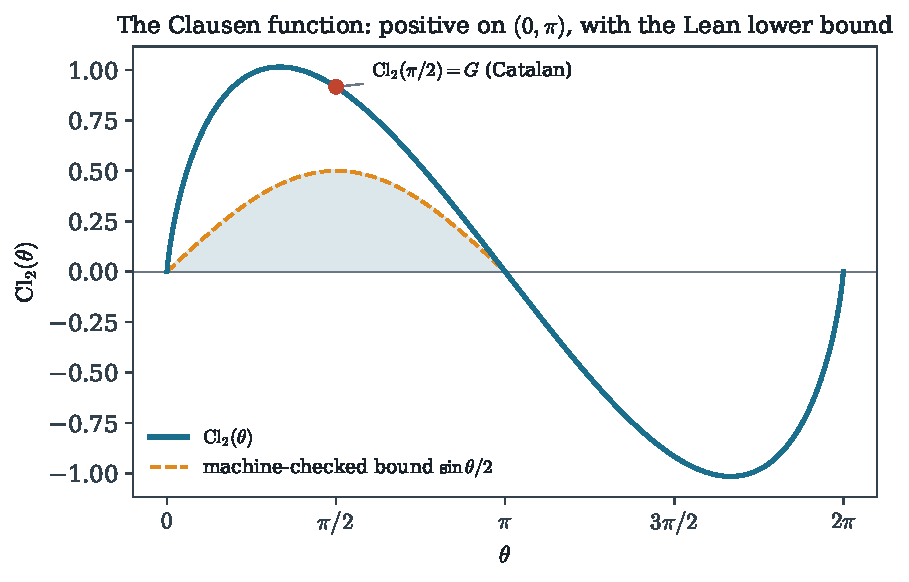
\includegraphics[width=0.78\textwidth]{dilog_fig2_clausen}
\caption{The Clausen function on $[0,2\pi]$ with the machine-checked lower bound
$\sin(\theta)/2$ (shaded) on $(0,\pi)$, and Catalan's constant at the quarter circle.
The generating script asserts the bound on a $400$-point grid at $30$ digits.}
\label{fig:clausen}
\end{figure}

\emph{From theory to practice.} The Fej\'er kernel underlies Ces\`aro summability of
Fourier series --- the standard remedy for Gibbs oscillation in signal reconstruction and
filter design --- and positivity of trigonometric partial sums is a recurring gate in
geometric function theory. The verified inequality is a reusable building block for
formalized approximation theory.

\emph{The turn --- the big one, and the honest one.} Step back and look at what we are
holding: a sum $\sum p_n e^{-in\theta}$ with positive weights $p_n\propto 1/n^2$, whose
imaginary part never vanishes on $(0,\pi)$. A physicist reads that expression instantly
--- it is the \emph{autocorrelation of a quantum state}, the inner product between a
state and its own time evolution, for populations $p_n$ on equally spaced energy
levels. We must be honest about how this reading entered the project, because it did
\emph{not} grow out of the chain of questions: a parallel thread --- born from asking
which part of the old ``universe as a computer'' metaphor is an actual theorem --- had
already formalized the two classical bounds on how fast any quantum state can evolve.
At this point the two threads crossed: the circle had been measuring \emph{time} all
along, and the positivity theorem we had just proved was a statement about a quantum
system that cannot reach an orthogonal state. What do the speed limits say about it?

\section{Q5: what physical thing beats to this function?}\label{sec:clock}

\emph{History bead.} Mandelstam and Tamm bounded the orthogonalization time by the
energy \emph{spread} in 1945~\cite{mandelstam}; Margolus and Levitin bounded it by the
mean energy in 1998~\cite{margolus}. Together they are the textbook ``quantum speed
limits'': how many distinguishable states can a system visit per unit time, on a given
energy budget. The Lean is \lean{QSL/}.

A state $\lvert\psi_0\rangle=\sum_n c_n\lvert E_n\rangle$ evolves with autocorrelation
$S(t)=\sum_n p_n e^{-iE_nt}$, $p_n=\lvert c_n\rvert^2$, and reaches an orthogonal state
at time $\tau$ iff $S(\tau)=0$. This is a statement about a scalar function of a
discrete nonnegative spectral measure, and that is how we formalize it --- the Hilbert
space is bookkeeping. Orthogonality enters as two real conditions
($\operatorname{Re}S=\operatorname{Im}S=0$); Margolus--Levitin needs no complex numbers
at all.

\begin{theorem}[{\lean{margolus\_levitin}, \lean{mandelstam\_tamm\_L1}}; $\hbar=1$]
\label{thm:qsl}
If $S(\tau)=0$ with $\tau\ge0$, then
\[
\pi \;\le\; 2\,\langle E\rangle\,\tau
\qquad\text{and}\qquad
1 \;\le\; D_1\,\tau,
\quad D_1=\textstyle\sum_n p_n\lvert E_n-\bar E\rvert .
\]
\end{theorem}

The heart of Margolus--Levitin is one inequality of independent interest,
$\cos x\ge 1-\tfrac{2}{\pi}(x+\sin x)$ for $x\ge0$ (equality at $0$ \emph{and} $\pi$),
which we prove by the same unimodal pattern as Fej\'er--Jackson: rise then fall, both
endpoints zero, split at $x_0=2\arctan(2/\pi)$. The same proof shape carried three
theorems in this paper --- that is not a coincidence but a transferable technique.
Since $D_1\le\Delta E$ by Cauchy--Schwarz, the second bound implies the textbook weak
Mandelstam--Tamm $\tau\ge1/\Delta E$; the sharp constant $\pi/2$ needs the geodesic
argument and is left as a road (\S\ref{sec:roads}).

Now the d\'enouement. Take populations $p_n=\frac{6}{\pi^2 n^2}$ on levels $E_n=n$: the
\emph{weight-2 zeta state}. Its autocorrelation \emph{is} our protagonist,
\[
S(\theta)=\frac{6}{\pi^2}\,\Li(e^{-i\theta})
=\frac{6}{\pi^2}\Big(
\underbrace{\tfrac{\pi^2}{6}-\tfrac{\pi\theta}{2}+\tfrac{\theta^2}{4}}_{\text{the
parabola of \S\ref{sec:circle}}}
\;-\;i\,\underbrace{\Cl(\theta)}_{\text{positive, by \S\ref{sec:fejer}}}\Big).
\]
Its mean energy $\sum_n p_n\,n$ \emph{diverges}. So does its energy variance. Both
bounds of Theorem~\ref{thm:qsl} are vacuously satisfied: on this state, the speed
limits of quantum mechanics predict nothing at all. We choose it on purpose --- it is
the bounds' blind spot, the regime where the textbook limits fall silent, and the
formalized dilogarithm is what answers in their place. One might guess such an
energy-unbounded state orthogonalizes instantly. The truth is the opposite extreme:

\begin{theorem}[{\lean{zetaState\_never\_orthogonal}}]\label{thm:clock}
For every $\theta\in(0,2\pi)$, the real and imaginary parts of the weight-2 zeta-state
autocorrelation are not both zero: the state \emph{never} reaches an orthogonal state.
\end{theorem}

\begin{proof}[Proof (as in Lean)]
On $(0,\pi)$ the imaginary part is $-\Cl(\theta)\ne0$ by the Fej\'er--Jackson bound. At
$\theta=\pi$ the real part is the parabola value $-\pi^2/12\ne0$ (it is $-\eta(2)$). On
$(\pi,2\pi)$, the reflection $\Cl(2\pi-\theta)=-\Cl(\theta)$ hands the sign back to the
first case.
\end{proof}

In fact $\lvert S\rvert\ge\frac{6}{\pi^2}\cdot\frac{\pi^2}{12}=\frac12$ on the whole
circle (certified numerically on a fine grid; the Lean theorem is the non-vanishing): the state never gets even \emph{halfway} to distinguishability
(Figure~\ref{fig:clock}). A clock with an infinite energy budget whose hand never
completes a tick --- because the budget is spent on a heavy spectral tail rather than
on coherent separation. Energy is necessary for evolution speed (Margolus--Levitin);
this is the machine-checked counterpoint that it is nowhere near sufficient.

\emph{From theory to practice.} Quantum speed limits set the minimum time for a gate, a
measurement, or a state transfer on a given energy budget; they recur across quantum
computing, metrology, and quantum thermodynamics (battery charging, optimal control).
The zeta state carries a practical lesson: a large energy budget buys no speed if it
sits in a heavy spectral tail --- fast evolution needs energy spread \emph{coherently},
not merely in quantity.

\begin{figure}[t]
\centering
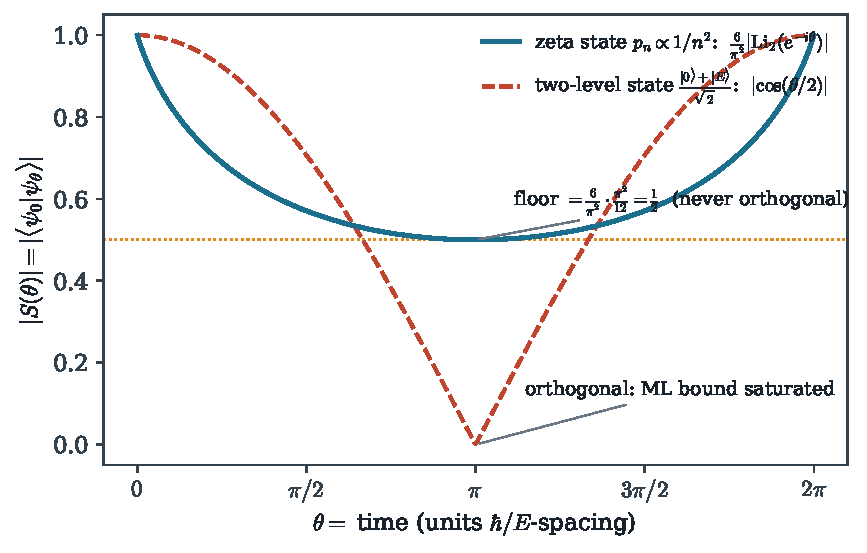
\includegraphics[width=0.82\textwidth]{dilog_fig3_clock}
\caption{Two states with the same level spacing. The two-level state
$(\lvert0\rangle+\lvert E\rangle)/\sqrt2$ (dashed) saturates Margolus--Levitin and
strikes orthogonality at $\theta=\pi$. The zeta state (solid), with \emph{infinite}
mean energy, has $\lvert S\rvert\ge\frac12$: the clock that never ticks. The script
asserts the floor equals $\eta(2)=\pi^2/12$ at $\theta=\pi$.}
\label{fig:clock}
\end{figure}

\begin{remark}[Which clocks do tick: a closing observation]\label{rem:ek}
For monotone non-increasing populations on equally spaced levels, ticking
(orthogonalization) means a zero of the power series $\sum_n p_nz^n$ \emph{on} the unit
circle. The Enestr\"om--Kakeya theorem (1893/1912)~\cite{enestrom} already forbids zeros
inside the disc; its boundary case pins down the rest. From
$(1-z)\sum_k p_kz^k=p_0+\sum_{k\ge1}(p_k-p_{k-1})z^k-p_Nz^{N+1}$, the triangle inequality
at $\lvert z\rvert=1$ is an equality only if every nonzero decrement $p_{k-1}-p_k$ sits
at an index $k$ with $z^k=1$: the decrements must concentrate on an arithmetic
progression, and the zero is a root of unity. The Margolus--Levitin--sharp state
$(\lvert0\rangle+\lvert E\rangle)/\sqrt2$ is exactly such a case ($\frac12(1+z)$, zero at
$z=-1$). The zeta state is the opposite extreme: its successive decrements
$p_n-p_{n+1}>0$ at \emph{every} index, never confined to a progression, so no root of
unity survives and the clock cannot tick --- recovering Theorem~\ref{thm:clock} from the
coefficient side. We have not found the resulting dictionary --- root location of
positive-coefficient series $\leftrightarrow$ orthogonalizability of monotone quantum
states --- in either literature; we record it as an observation and a road.
\end{remark}

\section{The boundary of the contribution}\label{sec:boundary}

Everything here that is mathematics is classical: Euler (1768), Landen (1780), Clausen
(1832), Rogers (1907), Fej\'er (1910), Jackson (1911), Mandelstam--Tamm (1945),
Margolus--Levitin (1998); the TBA reading of the golden values is from the 1990s. We
claim no new identity and no new inequality. The contributions are:
(i)~the machine-checked development itself --- per our checks of June 2026, the first
formalization in any proof assistant of each item listed in the abstract;
(ii)~three proof-engineering choices that may be reusable: the division-free Dirichlet
telescope, the asymptotics-free Abel bound $\Cl\ge\sin(\theta)/2$, and the fully real
(scalar spectral-measure) statements of the speed limits;
(iii)~the assembly of Theorem~\ref{thm:clock}, whose physical reading we have not seen
stated, though we would not be surprised to find it folklore among polylogarithm or QSL
specialists; and (iv)~the observation of Remark~\ref{rem:ek}.

\emph{Related formalization.} We build directly on Mathlib's analytic infrastructure:
term-by-term differentiation, the Weierstrass $M$-test, mean-value machinery, and the
Bernoulli--Fourier expansion that hands us the parabola for free. Special functions in
the proof-assistant literature have so far centred on $\Gamma$, $\zeta$, and the
elementary transcendental functions; the polylogarithms, the Clausen function, and
positive trigonometric sums were not among them. On the quantum side, the established
libraries (CoqQ, SQIR, Isabelle Marries Dirac) formalize circuits and gate semantics
rather than dynamical bounds on continuous evolution. This development sits in the gap
between those two bodies of work.

On methodology: the formalization was carried out in collaboration with an AI assistant
(Claude, Anthropic), with every step gated by the Lean kernel, every identity checked
independently at 20--50 digits \emph{before} formalization, and every named theorem
verified by \lean{\#print axioms} to depend only on \lean{propext},
\lean{Classical.choice}, \lean{Quot.sound}. Correctness does not rest on the assistant:
the Lean kernel checks every proof, so the AI affected the path to each theorem, not its
validity. The mathematics, the mistakes, and the claims remain the author's
responsibility.

\section{Open roads}\label{sec:roads}

\begin{enumerate}
\item \textbf{Abel's five-term relation} --- the capstone of weight 2; with it, every
two-variable dilogarithm identity follows. Our reflection/Landen machinery is the
warm-up.
\item \textbf{The complex dilogarithm} and the Bloch--Wigner function; with them, the
2D dimer entropy ($G/\pi$ --- Catalan again) and hyperbolic volumes come into reach.
\item \textbf{Sharp Mandelstam--Tamm} ($\pi/2\Delta E$, the geodesic argument) and the
arbitrary-fidelity Margolus--Levitin bound --- conjectured in 2003, proven only in
2023~\cite{hornedal}: a fresh theorem to formalize.
\item \textbf{Enestr\"om--Kakeya}, both as a formalization target and as the dictionary
of Remark~\ref{rem:ek}.
\item \textbf{Positive trigonometric sums beyond Fej\'er--Jackson} (Vietoris) --- the
toolkit is in place.
\end{enumerate}

\section*{Questions to take with you}

A paper built from questions should end with the ones it could not answer --- one per
station of the map, none of them rhetorical.

\begin{enumerate}
\item[\textbf{On Q1.}] Weight 1 (logarithms) needs no delicate limits; weight 2 needed
exactly one ($\ln x\cdot\ln(1-x)\to0$, the only place our formalization had to fight).
Is the number of genuinely delicate boundary limits an \emph{invariant of the weight}
--- and what does it count?

\item[\textbf{On Q2.}] We reached Landen's golden values by replacing one two-variable
identity (Abel's) with three one-variable ones, because the golden point sits where
reflection and Landen orbits intersect. Which specializations of the five-term relation
are reachable this way --- precisely: what is the subgroup of relations generated by
reflection, Landen and duplication inside the full functional-equation group of $\Li$,
and is the five-term relation in it?

\item[\textbf{On Q3.}] On the circle, the even-weight cosine series is a polynomial and
the sine series is transcendentally new; at odd weight the roles swap. What does weight
parity \emph{know} about the boundary that makes it exchange the tame and the wild
half?

\item[\textbf{On Q4.}] Three positivity proofs in this development share one shape:
rise-then-fall with both endpoints at zero (Fej\'er--Jackson, the Margolus--Levitin
cosine inequality, and $\Cl$ itself via the integral of $-\ln(2\sin(t/2))$). Is there a
single theorem behind them --- a maximum principle for positive sums --- of which all
three are instances, and would \emph{it} be the right thing to formalize next?

\item[\textbf{On Q5.}] The zeta state defeats both textbook speed limits through a
heavy spectral tail, yet its orthogonalization behaviour is perfectly determined. What
is the correct functional of the spectral measure that \emph{does} decide $\tau_\perp$
--- and is the Enestr\"om--Kakeya dictionary of Remark~\ref{rem:ek} its shadow on
monotone states?
\end{enumerate}

\appendix

\section{Reproducing}\label{app:repro}

\begin{verbatim}
git clone https://github.com/karlesmarin/godsil-gutman-lean
cd godsil-gutman-lean && lake exe cache get
lake build Dilog QSL
\end{verbatim}
Lean toolchain \lean{v4.30.0-rc2}, Mathlib pinned at \lean{701fb6e9}. The figures
regenerate with \lean{python figures/dilog\_fig*.py}; each script asserts its
mathematical content against 20--40-digit numerics before drawing.

\section{Lean inventory}

\begin{table}[H]
\centering\small
\begin{tabular}{@{}llr@{}}
\toprule
\rowcolor{ggteal!18} File & Contents & Lines\\
\midrule
\rowcolor{ggband!35} \lean{Dilog/Basic.lean} & $\Li$: series, derivative, reflection, Landen,&\\
\rowcolor{ggband!35} & duplication, $\Li(\frac12)$, golden ladder, Rogers $\Lrog$, Lee--Yang & 581\\
\lean{Dilog/Clausen.lean} & $\Cl$, Catalan's $G$, Bernoulli parabola, $\Cl\ge\sin\theta/2$,&\\
& $\Cl(2\pi-\theta)=-\Cl(\theta)$, Theorem~\ref{thm:clock} & 332\\
\rowcolor{ggband!35} \lean{Dilog/FejerJackson.lean} & Fej\'er--Jackson inequality & 189\\
\lean{QSL/Basic.lean} & Margolus--Levitin (+ the cosine inequality) & 238\\
\rowcolor{ggband!35} \lean{QSL/MandelstamTamm.lean} & Mandelstam--Tamm, $L^1$ form & 134\\
\midrule
&& 1\,474\\
\bottomrule
\end{tabular}
\caption{The development. All theorems \lean{sorry}-free; axioms:
\lean{propext}, \lean{Classical.choice}, \lean{Quot.sound} throughout.}
\label{tab:inventory}
\end{table}

\begin{thebibliography}{99}\small
\bibitem{lewin} L.~Lewin, \emph{Polylogarithms and Associated Functions}, North-Holland,
1981.
\bibitem{zagier} D.~Zagier, The dilogarithm function, in \emph{Frontiers in Number
Theory, Physics, and Geometry II}, Springer, 2007.
\bibitem{clausen} T.~Clausen, \"Uber die Function $\sin\varphi+\frac{1}{2^2}\sin2\varphi
+\frac{1}{3^2}\sin3\varphi+$ etc., \emph{J.\ Reine Angew.\ Math.} \textbf{8} (1832).
\bibitem{rogers} L.~J.~Rogers, On function sum theorems connected with the series
$\sum x^n/n^2$, \emph{Proc.\ London Math.\ Soc.} \textbf{4} (1907).
\bibitem{fejer} L.~Fej\'er, Lebesguesche Konstanten und divergente Fourierreihen,
\emph{J.\ Reine Angew.\ Math.} \textbf{138} (1910).
\bibitem{jackson} D.~Jackson, \"Uber eine trigonometrische Summe, \emph{Rend.\ Circ.\
Mat.\ Palermo} \textbf{32} (1911).
\bibitem{mandelstam} L.~Mandelstam and I.~Tamm, The uncertainty relation between energy
and time in nonrelativistic quantum mechanics, \emph{J.\ Phys.\ (USSR)} \textbf{9}
(1945) 249.
\bibitem{margolus} N.~Margolus and L.~B.~Levitin, The maximum speed of dynamical
evolution, \emph{Physica D} \textbf{120} (1998) 188; arXiv:quant-ph/9710043.
\bibitem{zamolodchikov} Al.~B.~Zamolodchikov, Thermodynamic Bethe ansatz in relativistic
models, \emph{Nucl.\ Phys.\ B} \textbf{342} (1990) 695.
\bibitem{nahm} W.~Nahm, Conformal field theory and torsion elements of the Bloch group,
in \emph{Frontiers in Number Theory, Physics, and Geometry II}, Springer, 2007.
\bibitem{kirillov} A.~N.~Kirillov, Dilogarithm identities, \emph{Prog.\ Theor.\ Phys.\
Suppl.} \textbf{118} (1995) 61.
\bibitem{enestrom} G.~Enestr\"om, \emph{\"Ofv.\ af Kungl.\ Vetenskaps-Akad.\ F\"orh.}
\textbf{50} (1893); S.~Kakeya, On the limits of the roots of an algebraic equation with
positive coefficients, \emph{T\^ohoku Math.\ J.} \textbf{2} (1912) 140.
\bibitem{hornedal} N.~H\"ornedal and O.~S\"onnerborn, The Margolus--Levitin quantum
speed limit for an arbitrary fidelity, \emph{Phys.\ Rev.\ Research} \textbf{5} (2023);
see also the elementary proof in arXiv:2307.16854.
\bibitem{alha} L.~Alha, Families of self-inverse functions and dilogarithm identities,
arXiv:2509.07598.
\bibitem{mathlib} The mathlib Community, The Lean mathematical library, \emph{CPP 2020}.
\end{thebibliography}

\end{document}
